\documentclass[10pt,a4paper]{article}
\usepackage[utf8]{inputenc}
\usepackage{amsmath}
\usepackage{amsfonts}	%Gestion dans les environnements mathématiques.
\usepackage{amssymb}
%\usepackage{bbm}		%Gestion des caractères pour les ensembles (N, Z, Q, R, C)
\usepackage{graphicx} 	%Gestion des images.
\usepackage{array}		%Gestion spécifique pour les tableaux.
						%Paramètres de placement dans les cellules: m, p, b. 
						%Avec dimensionnement de la colonne: m{2cm}.
\usepackage{multicol}	%Gère la mise en colonnes du texte.

\usepackage{fancyhdr}	%Gère la personnalisation des headers.
\usepackage{geometry}
\usepackage{marginnote}	%Gère la création de notes en marge du texte.
\usepackage{adjustbox}	%Options additionnelles de placement de l'image 
						%(left, right, center, outer and inner)
%-----------------------------------------------------------------------------
\title{Neural Networks}
\author{Lucas Wälti}
\date{\today}
%-----------------------------------------------------------------------------
\pagestyle{fancy} 	%Types de headers standards: empty, plain (default),
					%							 headings, myheadings, fancy.
\fancyhf{}			%Clear le header et footer par défaut.
\rhead{Theory}
\lhead{Neural Networks}	%Texte à droite, gauche et au centre du header.
\chead{}
\rfoot{}
\lfoot{}
\cfoot{Page \thepage}			%Texte du footer (ici: numéro de page).

\renewcommand{\headrulewidth}{0.5pt}
\renewcommand{\footrulewidth}{0pt}	%Lignes horizontales de séparation.
%-----------------------------------------------------------------------------
\begin{document}
\maketitle
\thispagestyle{empty}	%Supprime le header et le footer pour cette page. 

\newpage
\section{Introduction}
The following will try to provide an understanding of Convolution Neural Networks and of the mathematics behind this concept. The objective is to give a feeling of what is actually going on and of what is supervised learning.  
\subsection{The concept of Neuron}
The Neuron is the basic block of any Neural Network. A Neuron can receive any number of inputs $x_i$ and will apply a weight $w_i$ on each of these. The Net ($\sum_{i}{x_iw_i}$) is then created by adding those weighted inputs and is then evaluated by an activation function $f$ to produce an output $y$. 

\begin{figure}[h] %hbtp
\centering
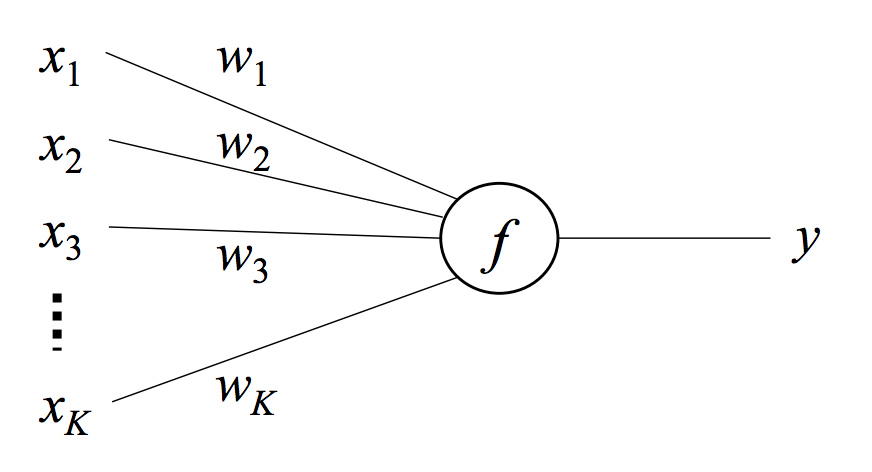
\includegraphics[scale=0.5]{neuron.png}
\caption{A single neuron}
\label{n}
\end{figure}

\subsection{The concept of Neural Network}
Neurons are then combined in layers and this is how a Neural Network could look like this: 

\begin{figure}[h] %hbtp
\centering
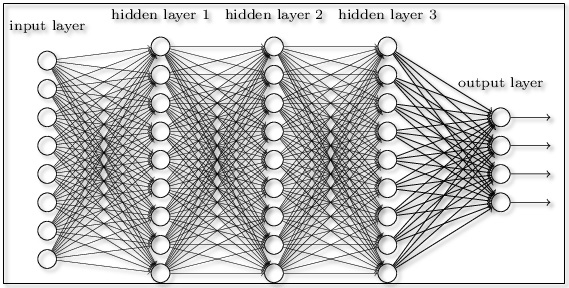
\includegraphics[scale=0.8]{NeuralNetwork.jpg}
\caption{A Neural Network}
\label{nn}
\end{figure}

\newpage
\section{The Backpropagation Problem}
To approach this problematic, it is necessary to start from the unit of the Network, i.e. the neuron, and then expand the development to the whole Network. 
\subsection{For a Single Neuron}
Let us first discuss how we can enable a single neuron to learn. We can observe that in figure \ref{n}, the inputs $In_i$ are each pondered by their corresponding weight $w_i$. Then the activation function $f$ will process everything and produce an output as described below. 

\begin{equation}\label{out}
out = f(\sum_{i}{w_i \cdot In_i}) = f(net)
\end{equation}

The activation function $f$ can be chosen among following functions: 

\begin{list}{•}{}
\item Sigmoid :  $ f(x) = \frac{1}{1 + e^{-\lambda(x - \theta)}} $
\item Tanh : $ f(x) = \tanh(\lambda(x - \theta)) $
\item Linear : $ f(x) = \lambda(x - \theta) $
\item ReLU (Rectified Linear Unit) : $ f(x) = \lambda(x - \theta)$ for $ x \geqslant 0 $, $ f(x) = 0 $ otherwise.
\item Leaky ReLU : $ f(x) = \lambda(x - \theta)$ for $ x \geqslant 0 $, $ f(x) = \epsilon \cdot \lambda(x - \theta) $ otherwise.
\end{list}

Where $\lambda$ and $\theta$ are usually 1 and 0 respectively and $\epsilon$ a small value. \\

Let us define the \textbf{Error} that the Neuron commits given a known input and output ($true$): 

\begin{equation}\label{Error}
E = (true - out)^2 
\end{equation}

The Error of equation \ref{Error} will be reduced by changing the value of the $i$ weights of the neuron through a gradient ($G_i$) descent: 

\[
G_i = \frac{\partial E }{\partial w_i} = \frac{\partial E }{\partial out} \cdot \frac{\partial out }{\partial w_i}
\]
with
$$
\frac{\partial E }{\partial out} = \frac{\partial}{\partial out}(true - out)^2 = -2(true - out)
$$ 
and 
$$
\frac{\partial out }{\partial w_i} = \frac{\partial}{\partial w_i}f(\sum_{j}w_j In_j) = In_i \cdot f'(net)
$$
Hence, the $i$ gradients of the $i$ weights are given by :
\begin{equation}\label{Gradient}
\boxed{G_i = -2(true - out)\frac{\partial f(\sum_{j}w_j In_j)}{\partial w_i}}
\end{equation}

An update step of the gradient descent happens then as follows: 
\begin{equation}\label{Update}
\boxed{w_i(t+1) = w_i(t) - \eta \cdot G_i}
\end{equation}

\newpage
\subsection{For a whole Network}

\begin{figure}[h] %hbtp
\centering
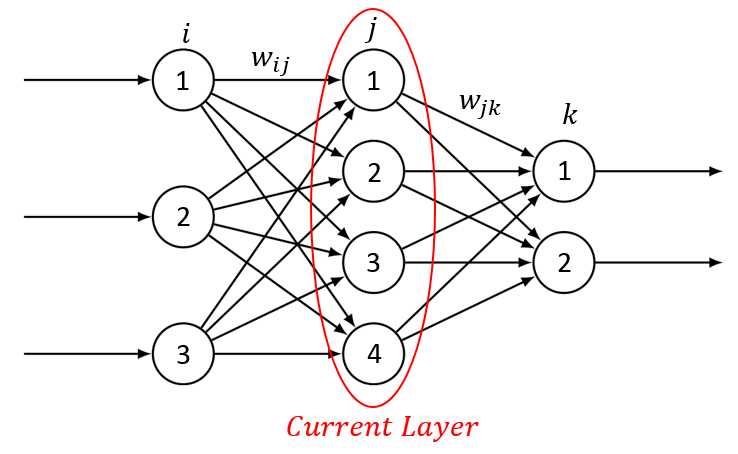
\includegraphics[scale=0.6]{3layers_detailed.png}
\caption{A Network with one hidden layer j}
\label{ref_nn}
\end{figure}

We will use the figure \ref{ref_nn} to build the equations we need to make any network learn. 
\paragraph{Error Signal of each Neuron} By definition, the error signal is given by
\begin{equation}\label{err_sig}
\delta_j = -\frac{\partial E_j}{\partial net_j}
\end{equation}
with the $net$ given by $net_j = \sum_{i}{w_{ij} \cdot out_i}$.

\paragraph{Inverted Gradient of Each Weight} The "inverted" gradient is defined in the same way it was for a single Neuron. 
$$
\Delta w_{ij} = -\frac{\partial E_j}{\partial w_{ij}}
			  = \underbrace{-\frac{\partial E_j}{\partial net_j}}_{\text{a)}} \cdot 
			    \underbrace{\frac{\partial net_j}{\partial w_{ij}}}_{\text{b)}}
$$
\begin{list}{}{}
\item a) $ -\frac{\partial E_j}{\partial net_j} = \delta_j $ by definition (see equation \ref{err_sig}). 
\item b) $ \frac{\partial net_j}{\partial w_{ij}} = \frac{\partial \sum_{i}{(w_{ij} \cdot out_i)}}{\partial w_{ij}} = out_i$
\end{list}

\begin{equation}\label{inv_grad}
\Rightarrow \boxed{\Delta w_{ij} = \delta_j \cdot out_i}
\end{equation}

\paragraph{Calculate Error Signal of Output Neuron(s)} The signal can be calculated as follows : 
$$
\delta_o = - \frac{\partial E}{\partial net} 
		 = - \frac{\partial}{\partial net}(t - out)^2
		 = - \frac{\partial}{\partial net}(t - f(net))^2
		 = - \frac{\partial f(net)}{\partial net} \cdot 2 \cdot (t - out)
$$
\begin{equation}\label{err_sig_o}
\Rightarrow \boxed{\delta_o = - \frac{\partial f(net)}{\partial net} \cdot 2 \cdot (t - out)}
\end{equation}

\paragraph{Backpropagate Error Signal} The error signal is then computed as follows for the rest of the Neurons. 
$$
\delta_j = - \frac{\partial E_j}{\partial net_j}
		 = \sum_{k}{- \frac{\partial E_k}{\partial net_k} \cdot
		   \frac{\partial net_k}{\partial out_j} \cdot
		   \frac{\partial out_j}{\partial net_j}}
		 = \sum_{k}{\delta_k \cdot w_{jk} \cdot \frac{\partial f(net_j)}{\partial net_j}}
$$
with 
$$
\frac{\partial net_k}{\partial out_j} = \frac{\partial \sum_{j}{w_{jk}out_j}}{\partial out_j} = w_{jk}
$$
hence
\begin{equation}\label{err_sig_all}
\Rightarrow \boxed{\delta_j = \frac{\partial f(net_j)}{\partial net_j} \cdot \sum_{k}{\delta_k \cdot w_{jk}}}
\end{equation}

Therefore the update step for any weight of the Neural Network is given by
\begin{equation}\label{net_update}
\Rightarrow 
\boxed{ 
	w_{ij}(t+1) = w_{ij}(t) + \eta \cdot \Delta w_{ij} 
				= w_{ij}(t) + \eta \cdot \delta_j \cdot out_i 
}
\end{equation}

\section{Some Good Practice}
\subsection{Weights Initialisation}
All weights should be very small non-zero values ($10^{-5} ~ 10^{-7}$). Typically for a sigmoid or tanh transfer function, the gradient will be computed where the slope is the potentially the greatest. 
\subsection{Input and Output Normalisation}
\begin{list}{•}{}
\item Output: The output does not necessarily need normalization. Typically, a linear activation function at the output does not require any normalization. If the output range is known, a normalization might be possible (between 0 and 1 or -1 and 1 for instance) but it is not recommended. 
\item Input: It is important to normalize the data (between 0 and 1 or -1 and 1 for instance, depending on the activation function chosen for the input layer). Furthermore, in case of multiple inputs, the data should be comparable. Being of the same unit is important but as well of having comparable range of values. Normalization can help with that. 
\end{list}
\subsection{Small Weight Updates}
The learning rate $\eta$ should be kept within the range $[0.001, 0.00001]$ typically. A possible behaviour during the learning process would be to see the error diminish and suddenly rise again. The error then does not change any more after that and it seems the network cannot learn. This is due to the fact that during the gradient descent, the weights overshoot their target values and then keep swinging around it because of the learning rate that is not small enough to provide a sufficiently precise learning. 

A solution to it is to decrease the value of the learning rate as a function of the number if iterations, which allows more and more precise gradient descent while not slowing down to much the learning process in the beginning. 
\subsection{Problem of local Minima}
The learning process can be blocked within a local minimum. The error stop reducing and does not tend to vary much anymore. The idea is to give a push to the network by adding a small random value to each of its weights to try and get it out of the minimum and hopefully allow it to keep learning. This process is called \textbf{Simulated Annealing} and is particularly of use in case of noisy data. 
\subsection{Network's Size}
There are no rule really on how to build a neural network. In order to choose how many layers and neurons should form the network, the following rule of thumb can be considered:
The size of the first hidden layer can be 1.5 to 2 times bigger then the input layer and slowly converges to the size of the output. 
\subsection{Over-fitting/Over-training}
In this scenario, the network has perfectly learn each points of its training set but is no longer capable of correctly generalize. That is why, training data has to be separated into a training set (70\%) and a testing set (30\%). It means that if the error of the training data keeps getting smaller but that at the same time, the error on the testing set rises, it means the network is becoming over-trained. A technique called \textbf{Early Stopping} consists to go back to the state of the network before the error on the testing set started getting greater. 

\end{document}